\documentclass[11pt,a4paper]{article}
\usepackage[margin=2.5cm]{geometry}
\usepackage{amsmath,amssymb}
\usepackage{booktabs}
\usepackage{array}
\newcolumntype{P}[1]{>{\raggedright\arraybackslash}p{#1}}
\usepackage{xcolor}
\usepackage{tcolorbox}
\tcbuselibrary{skins,breakable}
\usepackage{enumitem}
\usepackage{hyperref}
\usepackage[numbers,sort&compress]{natbib}
\bibliographystyle{unsrtnat}
\hypersetup{colorlinks=true,linkcolor=blue!60!black,urlcolor=blue!60!black}
\usepackage{tikz}
\usetikzlibrary{shapes.geometric,arrows.meta,decorations.pathmorphing,
                patterns,calc,positioning,shapes.arrows,fit,backgrounds}
\usepackage{pgfplots}
\pgfplotsset{compat=1.18}

\definecolor{boxblue}{RGB}{220,235,255}
\definecolor{boxorange}{RGB}{255,240,210}
\definecolor{boxgreen}{RGB}{220,245,220}
\definecolor{boxred}{RGB}{255,220,215}
\definecolor{boxgray}{RGB}{240,240,240}
% Vacuum colors for TikZ Kibble diagram
\definecolor{vacA}{RGB}{230,230,230}
\definecolor{vacB}{RGB}{200,220,255}
\definecolor{vacC}{RGB}{200,255,210}
\definecolor{vacD}{RGB}{255,250,200}
\definecolor{vacE}{RGB}{255,220,200}
\definecolor{vacF}{RGB}{240,200,255}
\definecolor{vacG}{RGB}{200,240,255}

\newcommand{\term}[1]{\textbf{#1}}
\newcommand{\PHIMDL}{\Phi_{\mathrm{MDL}}}
\newcommand{\TG}{T_G}
\newcommand{\ZS}{\mathbb{Z}_7}
\newcommand{\CatAL}{\textbf{CatAL}}
\newcommand{\CatAD}{\textbf{CatAD}}
\newcommand{\CatA}{\textbf{CatA}}

\title{\textbf{$\mathbb{Z}_7$ Defect Cosmology}\\[6pt]
\large Domain Walls, Phase Transitions, and the Zero-Relic Prediction\\[4pt]\normalsize\textit{UGP Physics Tutorial Series}
\\[2pt]\small\href{https://doi.org/\TutorialDOI}{doi.org/\TutorialDOI}}
\author{Nova Spivack\\[4pt]
\normalsize
\href{https://novaspivack.com/research}{novaspivack.com/research}\\[2pt]
\small Complete cosmology treatment (P47):
\href{https://doi.org/10.5281/zenodo.20560550}{doi.org/10.5281/zenodo.20560550}
}
\newcommand{\TutorialDOI}{10.5281/zenodo.20657866}
\date{2026}

\begin{document}
\setcounter{tocdepth}{2}
\maketitle
\tableofcontents
\newpage

\begin{tcolorbox}[colback=blue!6,colframe=blue!40!black,
  title=\textbf{UGP Physics Tutorial Series}]
\textbf{Prerequisites (read first):} \href{https://doi.org/10.5281/zenodo.20657864}{\emph{The Cosmological Constant}} $\cdot$ \href{https://doi.org/10.5281/zenodo.20657870}{\emph{Gravity from Description-Length Minimization}}\\[4pt]
\textbf{See also:} \href{https://doi.org/10.5281/zenodo.20657885}{\emph{The $\Phi_{\rm MDL}$ Field}}
\end{tcolorbox}

\begin{tcolorbox}[colback=boxgreen,colframe=green!50!black,
  title=\textbf{Claim-Strength Taxonomy}]
Throughout this tutorial, results are labeled with a confidence grade:
\begin{itemize}[itemsep=2pt]
  \item \textbf{$\mathbf{A}_{\rm Lean}$ (CatAL)} --- Machine-certified in Lean~4 with zero \texttt{sorry} and zero custom axioms.  Independently verifiable by anyone with Lean installed.
  \item \textbf{A/D (CatAD)} --- Analytically derived with full derivation, computationally confirmed.  Not yet machine-certified.
  \item \textbf{A (CatA)} --- Analytically derived; derivation complete but not independently machine-certified.
  \item \textbf{A/D (conditional)} --- Derived under a named, stated premise; the premise is itself an open problem or a CatB assumption.
  \item \textbf{B (CatB)} --- A stated working hypothesis or structural premise; not yet derived.
\end{itemize}
\end{tcolorbox}


%─────────────────────────────────────────────────────────────────────────────
\section{Phase Transitions in Cosmology}
%─────────────────────────────────────────────────────────────────────────────

\begin{tcolorbox}[colback=boxblue,colframe=blue!40!black,title=The one-line answer]
As the early universe cooled, it underwent phase transitions just like water
freezing into ice. When different regions of space independently ``chose'' their
low-temperature configuration, boundaries formed between them --- called
\emph{defects} or \emph{domain walls}. If stable, they would have been
catastrophic for the universe's development.
\end{tcolorbox}

\subsection{Water freezing: the everyday analogy}

When liquid water cools below $0^\circ$C, it freezes into ice.
In a large lake, the freezing does not happen all at once from a single point;
instead, tiny ice crystals nucleate simultaneously at many \emph{independent}
locations across the water.
Each crystal grows outward, but adjacent crystals were not in contact when they
started --- they independently chose their crystal orientation.
When the growing crystals meet, a boundary called a \term{grain boundary}
forms at their interface.
The grain boundary is a defect: a region where the crystal lattice is mismatched.

\medskip
\noindent
The same logic applies to the universe at cosmic scales.

\subsection{Phase transitions in the early universe}

Immediately after the Big Bang, the universe was unimaginably hot.
At those temperatures, all the symmetries of the laws of physics were
\emph{manifest}: particles and forces behaved in unified, symmetric ways.

As the universe expanded and cooled, it passed through a series of
\term{phase transitions} --- moments when the symmetric high-temperature
behaviour suddenly gave way to a broken-symmetry low-temperature configuration.
The most famous example is \emph{electroweak symmetry breaking} at about
$10^{15}$~K (roughly $100$~GeV in energy), when the photon and the weak gauge
bosons ($W$, $Z$) ``split apart'' from a unified electroweak field.

\begin{tcolorbox}[colback=boxorange,colframe=orange!60!black,title=Key idea: vacuum selection]
A phase transition happens when the system chooses a new \emph{ground state}
(lowest-energy configuration), called the \emph{vacuum}.
If the new ground state is not unique --- if several equally low-energy options
exist --- then different regions of space independently choose different options.
This is the origin of defects.
\end{tcolorbox}

\subsection{The defect zoo}

Different types of vacuum degeneracy produce different types of defects:

\begin{center}
\begin{tabular}{lll}
\toprule
Defect type & Origin & Dimensionality \\
\midrule
Cosmic strings & $U(1)$ vacuum degeneracy (a circle's worth of choices) & 1D lines \\
Domain walls & Discrete vacuum degeneracy (a finite set of choices) & 2D sheets \\
Monopoles & Higher-symmetry breaking & 0D points \\
\bottomrule
\end{tabular}
\end{center}

\medskip
\noindent
The GTE framework has a \emph{discrete} vacuum structure: the
$\PHIMDL$ field can sit in any of seven degenerate ground states,
indexed by elements of $\ZS = \{0, 1, 2, 3, 4, 5, 6\}$.
This leads to domain walls.

%─────────────────────────────────────────────────────────────────────────────
\section{The \texorpdfstring{$\mathbb{Z}_7$}{Z7} Domain-Wall Problem}
%─────────────────────────────────────────────────────────────────────────────

\begin{tcolorbox}[colback=boxblue,colframe=blue!40!black,
  title=The domain-wall problem in one sentence]
The GTE field $\PHIMDL$ has seven equally-valid ground states; if the universe
randomly populated them during a phase transition and they remained, stable
domain walls would have come to dominate the universe's energy budget ---
causing it to re-collapse. This is a known threat to any theory with multiple
discrete vacua.
\end{tcolorbox}

\subsection{The \texorpdfstring{$\PHIMDL$}{PhiMDL} field and its seven vacua}

The GTE framework is built around a physical field, written $\PHIMDL$, that
permeates all of space.
This field obeys a $\ZS$-symmetric potential --- a potential energy landscape
with \emph{seven equally-spaced minima} arranged like seven valleys on a ring.

\medskip
\noindent
\textbf{Vacuum $k=0$: the physical vacuum.}
Today the field sits everywhere in the ground state $k=0$ --- the
true physical vacuum.
Particles are not little balls floating in this field; they are
\emph{topological kinks}: regions where the field has permanently wound from
one vacuum sector to another.
An electron, for example, is a kink with winding number $w=4$
(the field changes from $k=0$ to $k=4$ as you cross the kink from left to right).

\medskip
\noindent
\textbf{Why seven?}
The number 7 is not chosen by hand.
It is selected by the Minimum Description Length (MDL) principle acting on the
arithmetic of the Generative Triple Evolution (GTE) sieve: among all prime
moduli, $|\ZS| = 7$ is the unique MDL-minimal choice consistent with the
Standard Model's fermion and generation structure.
The GTE polynomial $p(L,C,R) = C + R - CR - LCR \pmod{7}$ encodes all of this.

\subsection{The ordering crossover at \texorpdfstring{$T_G \approx 0.70$~GeV}{TG ≈ 0.70 GeV}}

At high temperature, thermal fluctuations are large enough to wash out the
distinctions between the seven vacua: the $\ZS$ symmetry is \emph{restored}.
As the universe cools, there is a critical temperature below which the
$\ZS$ order re-establishes itself.

For the $\PHIMDL$ field, the relevant criterion is \emph{Debye--Waller melting}.
The $\ZS$ order melts when thermal fluctuations exceed the spacing between vacua.
Setting the Debye--Waller condition, $\langle\varphi^2\rangle_T = T^2/12$,
the ordering-crossover temperature is:

\begin{tcolorbox}[colback=boxgreen,colframe=green!50!black,
  title={The GTE ordering-crossover temperature}]
\[
  T_G \approx 0.70~\text{GeV}
  \qquad
  \text{(normalization bracket } 0.70\text{--}1.24~\text{GeV})
\]
This temperature lies between the QCD scale ($\sim\!0.2$~GeV) and the
electroweak scale ($\sim\!100$~GeV).
It defines a new epoch in the GTE thermal history.
\end{tcolorbox}

\noindent
As the universe cools through $T_G$, the $\ZS$ vacuum is ``re-made'' locally
in each causally disconnected region of space independently.

\subsection{Why domain walls are fatal}

If different regions independently chose different vacua, and if no mechanism
existed to distinguish them, the following would happen:

\begin{enumerate}
\item A patchwork of domains forms, each in one of the seven vacua.
\item The boundaries between adjacent domains are domain walls --- 2D sheets
      of elevated potential energy.
\item A domain-wall network has an energy density $\rho_\mathrm{wall} \propto
      \sigma / t$, where $\sigma$ is the wall tension and $t$ is time.
\item In a flat universe, $\rho_\mathrm{wall}$ decays \emph{more slowly} than
      matter density ($\rho_m \propto t^{-2}$) or radiation density
      ($\rho_r \propto t^{-8/3}$).
\item Eventually, $\rho_\mathrm{wall}$ would come to dominate the total energy.
\end{enumerate}

For the $\PHIMDL$ field, the wall tension is fixed by the BPS kink integral:
\[
  \sigma = \tfrac{8}{49}\,m_\tau\,f^2 = 0.29010~\text{GeV}^3
  \quad (\text{canonical normalization}).
\]
An unbiased scaling network would come to dominate the energy budget at
\[
  z_\mathrm{dom} \approx 832 \qquad (T_\mathrm{dom} \approx 0.196~\text{eV}),
\]
exactly at the epoch of recombination ($z \approx 1100$).
This would violate the ZKO (Zel'\-dovich--Kobza\-rev--Okun) anisotropy bound
on CMB temperature variations by a factor of
$\approx 3.4 \times 10^3$: catastrophically too large.

\begin{tcolorbox}[colback=boxred,colframe=red!50!black,
  title={The catastrophe, quantified}]
An unbiased $\ZS$ domain-wall network would violate the CMB anisotropy bound
by a factor of $\approx 3400$ at recombination.
Every theory with discrete vacuum degeneracy must solve this problem.
This is the \textit{domain-wall problem}.
\end{tcolorbox}

%─────────────────────────────────────────────────────────────────────────────
\section{The Kibble Mechanism}
%─────────────────────────────────────────────────────────────────────────────

\begin{tcolorbox}[colback=boxblue,colframe=blue!40!black,title=Key idea]
The Kibble mechanism (Tom Kibble, 1976) explains why domain walls form whenever
a theory has multiple degenerate ground states and the universe undergoes a
phase transition.
It is a general causality argument: regions of space that were not in causal
contact at the phase transition could not have coordinated their vacuum choice.
\end{tcolorbox}

\subsection{Causal horizons in the early universe}

In the early universe, space was expanding so rapidly that distant regions had
never been in causal contact (no light signal could have traveled between them).
The \term{Hubble horizon} at any epoch is the characteristic scale over which
regions can communicate: roughly $c/H$, where $H$ is the Hubble rate.

At the ordering-crossover $T_G$, the Hubble horizon sets the coherence length:
\[
  \xi \sim \frac{1}{T_G} \approx \frac{1}{0.70~\text{GeV}}
  \approx 3\times10^{-16}~\text{m}.
\]
Regions separated by more than $\xi$ could not coordinate their vacuum
choice --- they independently and randomly picked one of the seven vacua.

\subsection{How the Kibble foam forms}

\begin{enumerate}
\item At $T > T_G$: $\ZS$ symmetry is restored; the field fluctuates
      uniformly among all sectors.
\item At $T = T_G$: each causal patch independently ``freezes'' into one
      of the seven vacua, with probability $\approx 1/7$ per vacuum.
\item Adjacent patches that froze into \emph{different} vacua are now
      separated by a domain wall.
\item The result is a complex, tangled foam of domain walls permeating
      all space.
\end{enumerate}

This foam is sometimes called \term{Kibble foam}.
For the $\ZS$ case, a lattice simulation confirms:
all seven vacua are populated at $\approx 1/7$ each,
six of the seven labels percolate (infinite walls are generic),
and $91\%$ of the wall area separates \emph{adjacent} vacua
(neighbouring $k$ values --- $|\Delta k| = 1$).

\subsection{A magnet analogy}

Imagine cooling a ferromagnet below its Curie temperature.
Each tiny domain independently aligns its spins along one of the available
magnetic directions.
Where two domains with opposite spin orientations meet, a domain wall forms.
The foam of magnetic domain walls that result is exactly the Kibble foam
in three-dimensional form.

In the cosmic case, the ``spin directions'' are replaced by the seven
$\ZS$ vacua, and the ``ferromagnet'' is the entire early universe.

%─────────────────────────────────────────────────────────────────────────────
\section{The GTE Resolution: Coupling-Bias Annihilation}
%─────────────────────────────────────────────────────────────────────────────

\begin{tcolorbox}[colback=boxblue,colframe=blue!40!black,
  title=The resolution in one sentence]
The $\PHIMDL$ Lagrangian contains a canonical coupling term that breaks the
exact $\ZS$ symmetry between the seven vacua, creating a tiny but nonzero
energy bias that drives the entire foam to collapse within
$\sim\!10^{-23}$~s --- long before any cosmological damage can occur.
\end{tcolorbox}

\subsection{Why a simple symmetry argument fails}

One might hope that the seven vacua, being exactly degenerate, would stay
exactly degenerate forever.
Inside the pure $\varphi$-sector of the $\PHIMDL$ field, this is indeed the case:
the $\ZS$ shift symmetry is exact to \emph{all orders} in perturbation theory,
and no bias can arise.
On its own, the vacuum energy cannot distinguish between $k = 0$, $k = 1$,
or any other vacuum label.
This means the catastrophe is not automatically avoided.

\subsection{The canonical coupling \texorpdfstring{$V_\mathrm{coupling}$}{V-coupling}}

The escape is provided by the \emph{full} Lagrangian of the theory.
The $\PHIMDL$ field does not live alone; it couples to a second field $\chi$
(the color sector), and the canonical coupling between them is:
\[
  V_\mathrm{coupling} = \varepsilon\,\varphi^2\,(D_\mu\chi)^2,
\]
where $\varepsilon = 7/9$ (machine-certified in Lean~4, zero \texttt{sorry}).
This coupling is \emph{not} $\ZS$-shift invariant.

\medskip
\noindent
\textbf{Why this breaks the symmetry.}
In vacuum $k$, the field value is $\varphi_k = $ (the field amplitude in
sector $k$).
Because the coupling involves $\varphi^2$, different vacua give different
values of $\varphi_k^2$, and thus different kinetic normalizations for the
$\chi$ field:
\[
  Z_k = 1 + 2\varepsilon\,\varphi_k^2, \qquad k = 0, 1, \ldots, 6.
\]
The vacuum $k = 0$ gives $Z_0 = 1$ (since $\varphi_0 = 0$ in the physical
vacuum); the other vacua give $Z_k > 1$.
This difference in kinetic normalization means the free energies of the
seven vacua are \emph{no longer equal} once the color sector is thermally
populated.

\subsection{The bias magnitude}

The vacuum-label splitting, computed from the
renormalization-group-improved effective potential anchored at the GTE
EFT boundary $\Lambda_\mathrm{GTE}$, is:
\begin{equation}
  |\Delta V(0\to 1)|(T_G) \approx 3.8 \times 10^{-2}~\text{GeV}^4
  \quad (\text{systematic battery: } 5\times10^{-4}\text{--}2\times10^{-1}),
  \label{eq:bias}
\end{equation}
of which $+2.8\times10^{-2}$~GeV$^4$ is a temperature-independent
Coleman--Weinberg component.
The annihilation does not even require the thermal window; the $T=0$
contribution alone is sufficient.

\begin{tcolorbox}[colback=boxorange,colframe=orange!60!black,title=Key numbers]
\begin{center}
\renewcommand{\arraystretch}{1.3}
\begin{tabular}{lll}
\toprule
Quantity & Value & Notes \\
\midrule
Wall tension $\sigma$ & $0.29010~\text{GeV}^3$ & From BPS kink integral \\
Bias $|\Delta V|$ & $3.8\times10^{-2}~\text{GeV}^4$ & RG-improved at $T_G$ \\
Critical radius $R_c$ & $7.7~\text{GeV}^{-1}$ & Above this, walls collapse \\
Foam lifetime $t_\mathrm{wall}$ & $\approx 5\times10^{-24}~\text{s}$ & Full collapse time \\
Annihilation temp.\ $T_\mathrm{ann}$ & $\approx T_G \approx 0.70$~GeV & Same epoch as formation \\
Margin before BBN & $\approx 700\times$ & Gone 700 times before nucleosynthesis \\
\bottomrule
\end{tabular}
\end{center}
\end{tcolorbox}

\subsection{The collapse: walls accelerate and annihilate}

Once the bias $|\Delta V|$ exists between adjacent vacua, a wall segment
feels a \emph{pressure difference} from either side.
The domain in the energetically preferred vacuum ($k = 0$) exerts more
pressure than the other side.
As long as the wall's curvature radius exceeds the critical value
$R_c = \sigma/\Delta V \approx 7.7~\text{GeV}^{-1}$, the wall accelerates
inward, converting the less-favored vacuum into the favored one.

The entire Kibble foam collapses with a characteristic time:
\[
  t_\mathrm{wall} \approx 5\times10^{-24}~\text{s}
  \;=\; 8\times10^{-18}\,H^{-1}(T_G).
\]
This is about $\sim 10^{-23}$~s total --- the universe was fully
``re-unified'' into the $k = 0$ vacuum within about one hundred-trillionth
of a trillionth of a second.

\medskip
\noindent
\textbf{The timeline.}
Big-Bang nucleosynthesis (BBN) --- the epoch when the lightest nuclei (hydrogen,
helium, lithium) formed --- occurs at $T_\mathrm{BBN} \approx 1~\text{MeV}$.
The domain walls annihilated at $T_\mathrm{ann} \approx 0.70$~GeV $\approx
700\,T_\mathrm{BBN}$: they were gone $700\times$ before the protons and neutrons
even began to fuse.

\subsection{Why the bias is ``the theory's own''}

This is the crucial structural point.
The coupling $V_\mathrm{coupling}$ is not added to the theory to solve the
domain-wall problem.
It is the \emph{canonical} coupling between the $\varphi$ and $\chi$ sectors
forced by the MDL uniqueness of the $\PHIMDL$ Lagrangian.
Its coefficient $\varepsilon = 7/9$ is derived, not fitted.
The resolution of the domain-wall problem is therefore \emph{automatic}: the
same coupling that is required for the particle spectrum and color sector
simultaneously annihilates the cosmological defect foam.

\begin{tcolorbox}[colback=boxgreen,colframe=green!50!black,
  title={Cross-level consistency remark}]
At Level~1 (algebraic certificate), the CA fixed-point theorem establishes
that $k = 0$ is the unique fixed point of the $p$-dynamics at every ring size
(\texttt{vacuum\_unique\_temporal\_fixed\_point\_ring}, \CatAL{}).
At Level~2 (continuum field), the RG-improved effective potential also selects
$k = 0$ across the full systematic battery.
The algebraic structure and the thermodynamic bias independently converge on
the same vacuum.
\end{tcolorbox}

%─────────────────────────────────────────────────────────────────────────────
\section{The Kibble Foam: A TikZ Diagram}
%─────────────────────────────────────────────────────────────────────────────

The sequence below illustrates the formation and annihilation of the Kibble foam.

\begin{center}
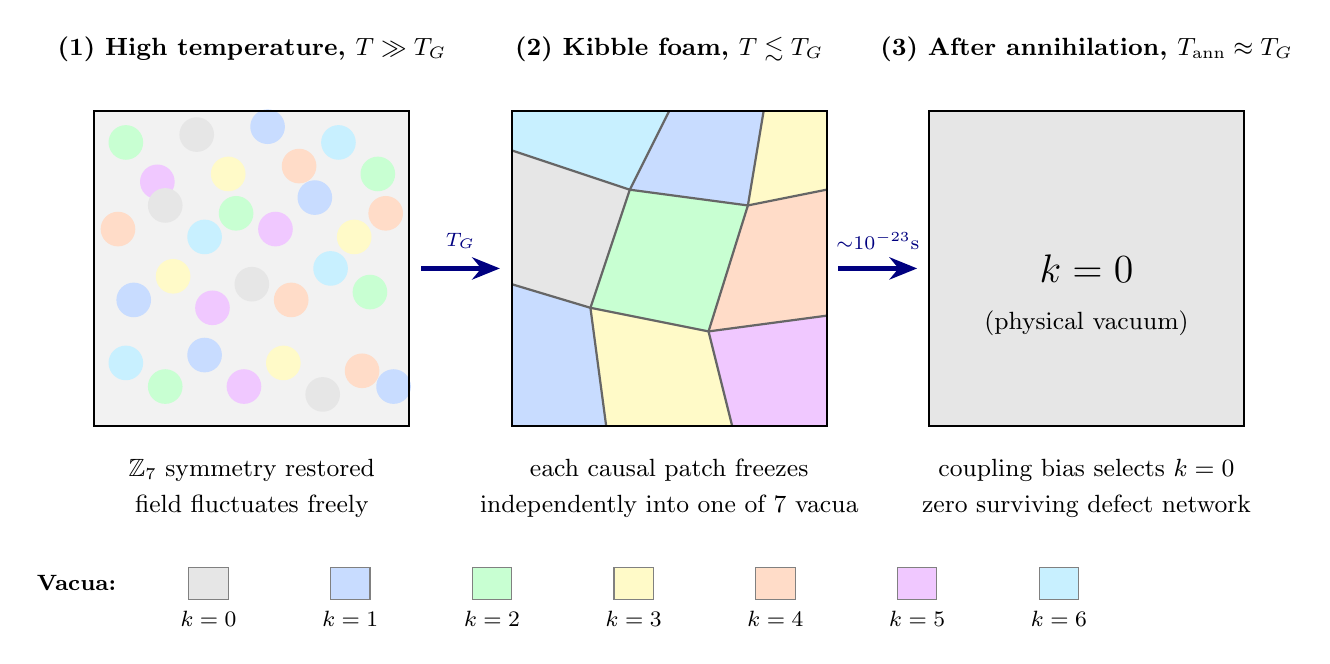
\begin{tikzpicture}[font=\small]

%─── Stage 1: high temperature, disordered ───────────────────────────────────
\begin{scope}[xshift=0cm]
  \node[above] at (2,4.5) {\textbf{(1) High temperature, $T \gg T_G$}};
  \node[below] at (2,-0.3) {$\ZS$ symmetry restored};
  \node[below] at (2,-0.75) {field fluctuates freely};
  \fill[gray!10] (0,0) rectangle (4,4);
  % Scattered dots showing thermal disorder among 7 vacua
  \fill[fill=vacC] (0.4,3.6) circle (0.22);
  \fill[fill=vacF] (0.8,3.1) circle (0.22);
  \fill[fill=vacA] (1.3,3.7) circle (0.22);
  \fill[fill=vacD] (1.7,3.2) circle (0.22);
  \fill[fill=vacB] (2.2,3.8) circle (0.22);
  \fill[fill=vacE] (2.6,3.3) circle (0.22);
  \fill[fill=vacG] (3.1,3.6) circle (0.22);
  \fill[fill=vacC] (3.6,3.2) circle (0.22);
  \fill[fill=vacE] (0.3,2.5) circle (0.22);
  \fill[fill=vacA] (0.9,2.8) circle (0.22);
  \fill[fill=vacG] (1.4,2.4) circle (0.22);
  \fill[fill=vacC] (1.8,2.7) circle (0.22);
  \fill[fill=vacF] (2.3,2.5) circle (0.22);
  \fill[fill=vacB] (2.8,2.9) circle (0.22);
  \fill[fill=vacD] (3.3,2.4) circle (0.22);
  \fill[fill=vacE] (3.7,2.7) circle (0.22);
  \fill[fill=vacB] (0.5,1.6) circle (0.22);
  \fill[fill=vacD] (1.0,1.9) circle (0.22);
  \fill[fill=vacF] (1.5,1.5) circle (0.22);
  \fill[fill=vacA] (2.0,1.8) circle (0.22);
  \fill[fill=vacE] (2.5,1.6) circle (0.22);
  \fill[fill=vacG] (3.0,2.0) circle (0.22);
  \fill[fill=vacC] (3.5,1.7) circle (0.22);
  \fill[fill=vacG] (0.4,0.8) circle (0.22);
  \fill[fill=vacC] (0.9,0.5) circle (0.22);
  \fill[fill=vacB] (1.4,0.9) circle (0.22);
  \fill[fill=vacF] (1.9,0.5) circle (0.22);
  \fill[fill=vacD] (2.4,0.8) circle (0.22);
  \fill[fill=vacA] (2.9,0.4) circle (0.22);
  \fill[fill=vacE] (3.4,0.7) circle (0.22);
  \fill[fill=vacB] (3.8,0.5) circle (0.22);
  \draw[thick] (0,0) rectangle (4,4);
\end{scope}

%─── Stage 2: just below TG, foam forms ──────────────────────────────────────
\begin{scope}[xshift=5.3cm]
  \node[above] at (2,4.5) {\textbf{(2) Kibble foam, $T \lesssim T_G$}};
  \node[below] at (2,-0.3) {each causal patch freezes};
  \node[below] at (2,-0.75) {independently into one of 7 vacua};
  \fill[gray!10] (0,0) rectangle (4,4);
  \fill[fill=vacB] (0,0) -- (1.2,0) -- (1.0,1.5) -- (0,1.8) -- cycle;
  \fill[fill=vacD] (1.2,0) -- (2.8,0) -- (2.5,1.2) -- (1.0,1.5) -- cycle;
  \fill[fill=vacF] (2.8,0) -- (4,0) -- (4,1.4) -- (2.5,1.2) -- cycle;
  \fill[fill=vacA] (0,1.8) -- (1.0,1.5) -- (1.5,3.0) -- (0,3.5) -- cycle;
  \fill[fill=vacC] (1.0,1.5) -- (2.5,1.2) -- (3.0,2.8) -- (1.5,3.0) -- cycle;
  \fill[fill=vacE] (2.5,1.2) -- (4,1.4) -- (4,3.0) -- (3.0,2.8) -- cycle;
  \fill[fill=vacG] (0,3.5) -- (1.5,3.0) -- (2.0,4.0) -- (0,4) -- cycle;
  \fill[fill=vacB] (1.5,3.0) -- (3.0,2.8) -- (3.2,4.0) -- (2.0,4.0) -- cycle;
  \fill[fill=vacD] (3.0,2.8) -- (4,3.0) -- (4,4) -- (3.2,4.0) -- cycle;
  \draw[thick,black!60] (1.2,0) -- (1.0,1.5);
  \draw[thick,black!60] (2.8,0) -- (2.5,1.2);
  \draw[thick,black!60] (1.0,1.5) -- (2.5,1.2);
  \draw[thick,black!60] (0,1.8) -- (1.0,1.5);
  \draw[thick,black!60] (2.5,1.2) -- (4,1.4);
  \draw[thick,black!60] (1.0,1.5) -- (1.5,3.0);
  \draw[thick,black!60] (2.5,1.2) -- (3.0,2.8);
  \draw[thick,black!60] (1.5,3.0) -- (3.0,2.8);
  \draw[thick,black!60] (0,3.5) -- (1.5,3.0);
  \draw[thick,black!60] (3.0,2.8) -- (4,3.0);
  \draw[thick,black!60] (1.5,3.0) -- (2.0,4.0);
  \draw[thick,black!60] (3.0,2.8) -- (3.2,4.0);
  \draw[thick] (0,0) rectangle (4,4);
\end{scope}

%─── Stage 3: after annihilation ─────────────────────────────────────────────
\begin{scope}[xshift=10.6cm]
  \node[above] at (2,4.5) {\textbf{(3) After annihilation, $T_\mathrm{ann} \approx T_G$}};
  \node[below] at (2,-0.3) {coupling bias selects $k=0$};
  \node[below] at (2,-0.75) {zero surviving defect network};
  \fill[fill=vacA] (0,0) rectangle (4,4);
  \node[font=\Large] at (2,2) {$k=0$};
  \node at (2,1.3) {(physical vacuum)};
  \draw[thick] (0,0) rectangle (4,4);
\end{scope}

%─── Time arrows ─────────────────────────────────────────────────────────────
\draw[-{Stealth[length=10pt,width=8pt]},line width=2pt,blue!50!black]
  (4.15,2) -- (5.15,2);
\draw[-{Stealth[length=10pt,width=8pt]},line width=2pt,blue!50!black]
  (9.45,2) -- (10.45,2);
\node[blue!50!black,font=\scriptsize] at (4.65,2.35) {$T_G$};
\node[blue!50!black,font=\scriptsize] at (9.95,2.35) {${\sim}10^{-23}$s};

%─── Color legend ────────────────────────────────────────────────────────────
\begin{scope}[xshift=0cm, yshift=-2.2cm]
  \node[left,font=\footnotesize\bfseries] at (0.4,0.2) {Vacua:};
  \fill[fill=vacA] (1.2,0.0) rectangle (1.7,0.4);
  \draw[black!50] (1.2,0.0) rectangle (1.7,0.4);
  \node[font=\footnotesize] at (1.45,-0.25) {$k=0$};
  \fill[fill=vacB] (3.0,0.0) rectangle (3.5,0.4);
  \draw[black!50] (3.0,0.0) rectangle (3.5,0.4);
  \node[font=\footnotesize] at (3.25,-0.25) {$k=1$};
  \fill[fill=vacC] (4.8,0.0) rectangle (5.3,0.4);
  \draw[black!50] (4.8,0.0) rectangle (5.3,0.4);
  \node[font=\footnotesize] at (5.05,-0.25) {$k=2$};
  \fill[fill=vacD] (6.6,0.0) rectangle (7.1,0.4);
  \draw[black!50] (6.6,0.0) rectangle (7.1,0.4);
  \node[font=\footnotesize] at (6.85,-0.25) {$k=3$};
  \fill[fill=vacE] (8.4,0.0) rectangle (8.9,0.4);
  \draw[black!50] (8.4,0.0) rectangle (8.9,0.4);
  \node[font=\footnotesize] at (8.65,-0.25) {$k=4$};
  \fill[fill=vacF] (10.2,0.0) rectangle (10.7,0.4);
  \draw[black!50] (10.2,0.0) rectangle (10.7,0.4);
  \node[font=\footnotesize] at (10.45,-0.25) {$k=5$};
  \fill[fill=vacG] (12.0,0.0) rectangle (12.5,0.4);
  \draw[black!50] (12.0,0.0) rectangle (12.5,0.4);
  \node[font=\footnotesize] at (12.25,-0.25) {$k=6$};
\end{scope}

\end{tikzpicture}
\end{center}

\medskip
\noindent
In stage (2), the thick black lines are domain walls --- boundaries between regions
that froze into different vacua.
In stage (3), the coupling bias has driven all domains to collapse into $k = 0$;
the walls have annihilated.
This happens within $\sim 10^{-23}$~s, far before any cosmological epoch of
interest.

%─────────────────────────────────────────────────────────────────────────────
\section{The Falsifiable Prediction}
%─────────────────────────────────────────────────────────────────────────────

\begin{tcolorbox}[colback=boxblue,colframe=blue!40!black,title=Key idea]
Because the wall tension $\sigma$ and the annihilation temperature $T_\mathrm{ann}$
are both \emph{parameter-free} (derived from first principles with no free
parameters fitted), the relic inventory is sharp: zero surviving defect network,
with a specific gravitational-wave ceiling and a specific neutrino-sector
prediction.
These are falsifiable: any confirmed domain-wall relic would rule out the
GTE defect-cosmology mechanism.
\end{tcolorbox}

\subsection{What ``zero surviving network'' means}

The zero-relic prediction means:
\begin{itemize}
\item \textbf{No domain walls survive} to Big-Bang nucleosynthesis (BBN),
      to the epoch of recombination, or to today.
\item \textbf{No stochastic gravitational-wave background} from domain walls:
      the foam never reaches the scaling regime in which it would radiate
      gravitational waves at observable levels.
\item \textbf{No extra relativistic species}: the transient foam carries at most
      $4.2\%$ of the radiation density for only $\sim 10^{-22}$~s before
      rethermalizing into Standard-Model quanta, giving $\Delta N_\mathrm{eff}
      \approx 0$ --- well within current observational bounds.
\end{itemize}

\subsection{The gravitational-wave ceiling}

The most precisely quantified prediction is the \term{GW ceiling}:
the upper bound on the stochastic gravitational-wave background from this
domain-wall sector.
Because the walls annihilate before entering the scaling regime, the
gravitational-wave signal is bounded by the energy density of the
transient foam at the moment of annihilation:

\begin{tcolorbox}[colback=boxgreen,colframe=green!50!black,
  title={Gravitational-wave ceiling (GTE zero-relic prediction)}]
\[
  \Omega_\mathrm{GW}\,h^2 \;\lesssim\; 3\times10^{-47}
  \quad\text{at}\quad f \approx 0.02~\text{Hz}
\]
This is in the LISA frequency band, but approximately $25$ orders of magnitude
below LISA's sensitivity threshold ($\Omega_\mathrm{GW} h^2 \sim 10^{-12}$
at that frequency).
GTE predicts that \emph{any} common-spectrum stochastic gravitational-wave
process seen by pulsar-timing arrays or LISA is \textbf{not} from this
$\ZS$ domain-wall sector.
\end{tcolorbox}

\subsection{Falsification criteria}

\begin{center}
\begin{tabular}{P{3.8cm} P{4.5cm} P{5.0cm}}
\toprule
\textbf{Prediction} & \textbf{Value / bound} & \textbf{How to falsify} \\
\midrule
Zero relic network & No domain-wall relics to BBN & Detection of a cosmological
  domain-wall relic at any epoch \\[6pt]
GW ceiling & $\Omega_\mathrm{GW} h^2 \lesssim 3\times10^{-47}$ at $0.02$~Hz &
  Confirmed detection of a GW stochastic background attributed to a
  $\ZS$-type domain-wall sector \\[6pt]
$\Delta N_\mathrm{eff}$ & $\approx 0$ (no extra relativistic species) &
  CMB-S4 or Simons Observatory precision measurement $\Delta N_\mathrm{eff}
  > 0.1$ attributable to domain walls \\[6pt]
Vacuum selected & $k^* = 0$ (unique) & Any observation implying residual
  $\ZS$ vacuum degeneracy in the present-day universe \\
\bottomrule
\end{tabular}
\end{center}

\noindent
What would \emph{not} be falsified by a domain-wall relic detection:
the substrate identification ($\PHIMDL$ as the physical field), the particle
spectrum derivations, the GTE polynomial, or the broader derivation tower.
The detection would falsify specifically the coupling-bias annihilation
mechanism and the ordering-crossover epoch, requiring a different resolution
of the domain-wall problem.

%─────────────────────────────────────────────────────────────────────────────
\section{Why This Is Remarkable}
%─────────────────────────────────────────────────────────────────────────────

\begin{tcolorbox}[colback=boxblue,colframe=blue!40!black,
  title=The three-sentence summary]
Any theory with discrete vacuum degeneracy faces the domain-wall problem.
GTE resolves it dynamically, using its own canonical coupling rather than by
imposing an extra assumption.
The resolution is testable: it predicts zero surviving defect network and a
specific gravitational-wave ceiling, both falsifiable by current-generation
experiments.
\end{tcolorbox}

\subsection{The domain-wall problem as a consistency test}

The domain-wall problem is not a peripheral worry.
For any theory that:
\begin{enumerate}
\item Has multiple degenerate discrete ground states, \emph{and}
\item Claims to describe the early universe's thermal history, \emph{and}
\item Has no built-in mechanism to remove the walls,
\end{enumerate}
\noindent
a cosmological domain-wall catastrophe is \emph{guaranteed}.
The problem was first clearly articulated by Zel'dovich, Kobzarev, and Okun
in 1974 (Zel'dovich, Kobzarev, Okun; see Further Reading).
Any new physics beyond the Standard Model that introduces discrete symmetry
breaking faces the same hurdle.

\subsection{Three approaches to resolution}

There are three broad strategies for solving the domain-wall problem:

\begin{center}
\begin{tabular}{lP{5.0cm}P{5.0cm}}
\toprule
\textbf{Strategy} & \textbf{How it works} & \textbf{Cost} \\
\midrule
\textbf{Inflation} & Walls form before inflation, which dilutes them
  exponentially. & Requires a separate inflationary mechanism (absent in GTE,
  which predicts $r=0$). \\[6pt]
\textbf{Explicit breaking} & Add a term to the potential that explicitly
  breaks the discrete symmetry from the start. & Requires a new free parameter
  or a new theoretical input; not self-contained. \\[6pt]
\textbf{Bias annihilation} & A small energy bias between vacua drives walls to
  collapse dynamically. & None, if the bias is already present in the canonical
  Lagrangian. \emph{This is the GTE mechanism.} \\
\bottomrule
\end{tabular}
\end{center}

\medskip
\noindent
GTE uses the third strategy, but without introducing any new input: the
coupling $V_\mathrm{coupling} = \varepsilon\varphi^2(D_\mu\chi)^2$ is
already present in the canonical Lagrangian, with $\varepsilon = 7/9$
fixed by MDL minimality.
The resolution is not engineered; it is discovered.

\subsection{The falsifiable nature of the prediction}

Most cosmological defect scenarios are theoretically well-motivated but
difficult to make precise: the size of the bias, the moment of annihilation,
and the relic density depend on model parameters that can be tuned.
In GTE, there are no tunable parameters.
The wall tension is fixed by the BPS kink integral; the bias is fixed by the
coupling coefficient $\varepsilon = 7/9$ and the color sector running; the
annihilation temperature is $T_\mathrm{ann} \approx T_G \approx 0.70$~GeV.
The GW ceiling $\Omega_\mathrm{GW} h^2 \lesssim 3\times10^{-47}$ follows.

This sharpness is what distinguishes a \emph{prediction} from a
\emph{postdiction}.
If LISA were to detect a stochastic gravitational-wave background at $0.02$~Hz
above the $3\times10^{-47}$ ceiling, that specific number would be falsified
--- not merely challenged, but contradicted by a first-principles derivation.

\subsection{Connection to the broader GTE picture}

The domain-wall resolution is part of a cluster of zero-parameter
cosmological predictions:

\begin{center}
\begin{tabular}{P{3.6cm} P{4.0cm} P{4.5cm}}
\toprule
\textbf{Observable} & \textbf{GTE prediction} & \textbf{Agreement} \\
\midrule
CMB spectral tilt $n_s$ & $1 - \ln 2/(2\pi^2) = 0.96488$ & $-0.005\sigma$
  vs.\ Planck 2018 \\[4pt]
Baryon asymmetry $\eta_B$ & $6.109\times10^{-10}$ & $+0.15\sigma$
  vs.\ Planck 2018 CMB+BBN \\[4pt]
$\ZS$ defect relic & Zero surviving network & No domain-wall relic
  observed (consistent) \\[4pt]
GW ceiling (walls) & $\lesssim 3\times10^{-47}$ at $0.02$~Hz &
  Not yet tested (far below LISA) \\[4pt]
Dark energy eq.\ of state & $w_0 = -1$ exactly, $w_a = 0$ & DESI Year-1
  at $1.37\sigma$ (consistent) \\[4pt]
Tensor-to-scalar ratio $r$ & $0$ (no primordial GWs) & Current upper limit
  $r < 0.036$ (consistent) \\
\bottomrule
\end{tabular}
\end{center}

\medskip
\noindent
All predictions carry zero free parameters.
The domain-wall prediction fits naturally within a framework that derives ---
rather than postulates --- the thermal history of the universe.

\bigskip
\begin{tcolorbox}[colback=boxblue,colframe=blue!40!black,
  title=One-paragraph summary of the Z7 defect-cosmology result]
The $\PHIMDL$ field has seven equally-spaced degenerate ground states
($\ZS$ vacua).
When the universe cooled through the ordering crossover $T_G \approx
0.70$~GeV, independent causal regions chose different vacua (the Kibble
mechanism), forming a domain-wall foam.
Without a bias, this foam would have dominated the universe's energy at
recombination --- catastrophic.
The GTE Lagrangian's canonical coupling term $\varepsilon\varphi^2(D_\mu\chi)^2$
($\varepsilon = 7/9$, derived) provides exactly such a bias: the vacuum-label
splitting $|\Delta V| \approx 3.8\times10^{-2}~\text{GeV}^4$ drives the
entire foam to annihilate within $\sim 10^{-23}$~s, $700\times$ before BBN,
selecting the unique vacuum $k = 0$.
This leaves zero surviving defect network --- a parameter-free falsifiable
prediction with a specific gravitational-wave ceiling
$\Omega_\mathrm{GW} h^2 \lesssim 3\times10^{-47}$ at $f \approx 0.02$~Hz.
\end{tcolorbox}

%─────────────────────────────────────────────────────────────────────────────
\appendix
\section{Quick Reference: Timeline and Scales}
%─────────────────────────────────────────────────────────────────────────────

\begin{center}
\begin{tabular}{P{3.8cm} P{3.2cm} P{5.5cm}}
\toprule
\textbf{Epoch} & \textbf{Temperature} & \textbf{What happens} \\
\midrule
Reheating (post-bounce) & $6.49\times10^8$~GeV & Universe filled with $\PHIMDL$
  excitations in thermal equilibrium; $\ZS$ order is disordered \\[4pt]
$\ZS$ ordering crossover & $T_G \approx 0.70$~GeV & Kibble foam forms; all
  7 vacua populated at $\approx 1/7$ each \\[4pt]
Foam annihilation & $T_\mathrm{ann} \approx T_G$ & Coupling bias collapses
  foam within $\sim 5\times10^{-24}$~s \\[4pt]
QCD crossover & $\sim 0.15$~GeV & Quarks confine into hadrons \\[4pt]
Big-Bang nucleosynthesis & $\sim 1$~MeV & H, He, Li nuclei form;
  walls were gone $\sim 700\times$ earlier \\[4pt]
Recombination & $\sim 0.25$~eV & CMB photons decouple;
  domain-wall catastrophe would have occurred here without the bias \\[4pt]
Today & $2.7\times10^{-4}$~eV & Zero surviving defect network \\
\bottomrule
\end{tabular}
\end{center}

%─────────────────────────────────────────────────────────────────────────────
\section{Additional References}
%─────────────────────────────────────────────────────────────────────────────

\begin{itemize}
\item \textbf{Full derivation of GTE defect cosmology:}
  P47~\cite{SpivackGTECosmology} --- ``GTE Cosmological Predictions'' (Nova Spivack, 2026).
  \href{https://doi.org/10.5281/zenodo.20465803}{doi.org/10.5281/zenodo.20465803}

\item \textbf{The $\PHIMDL$ field and its Lagrangian:}
  P42 --- ``The $\Phi_\mathrm{MDL}$ Field.''
  \\\url{https://doi.org/10.5281/zenodo.20417576}

\item \textbf{The complete GTE monograph:}
  P48~\cite{SpivackGTECompleteFramework} --- ``GTE: The Complete Theory'' (Nova Spivack, 2026).
  \href{https://doi.org/10.5281/zenodo.20560550}{doi.org/10.5281/zenodo.20560550}

\item \textbf{GTE polynomial tutorial:}
  ``The GTE Polynomial: A Step-by-Step Cheat Sheet''
  (companion tutorial in this series).

\item \textbf{Original domain-wall problem:}
  Ya.B.~Zel'dovich, I.Yu.~Kobzarev, L.B.~Okun,
  Zh.\ Eksp.\ Teor.\ Fiz.\ \textbf{67}, 3 (1974).

\item \textbf{Kibble mechanism:}
  T.W.B.~Kibble, J.\ Phys.\ A \textbf{9}, 1387 (1976).

\item \textbf{LISA gravitational-wave observatory:}
  P.\ Amaro-Seoane et al., arXiv:1702.00786 (2017).
\end{itemize}


\section*{Further Reading}
\begin{tcolorbox}[colback=orange!8,colframe=orange!50!black,
  title=\textbf{Primary Sources}]
The results in this tutorial are derived in the following papers,
all available open-access on Zenodo and at
\href{https://novaspivack.com/research}{novaspivack.com/research}:
\begin{itemize}
  \item \textbf{P47 --- GTE Cosmological Predictions} (defect cosmology, relic constraints):\\
        \href{https://doi.org/10.5281/zenodo.20465803}{doi.org/10.5281/zenodo.20465803}
  \item \textbf{P42 --- The $\Phi_{\rm MDL}$ Field} (kink/domain-wall spectrum):\\
        \href{https://doi.org/10.5281/zenodo.20417576}{doi.org/10.5281/zenodo.20417576}
  \item \textbf{P48 --- The Complete GTE Framework} (main synthesis monograph):\\
        \href{https://doi.org/10.5281/zenodo.20560550}{doi.org/10.5281/zenodo.20560550}
\end{itemize}
Lean~4 machine proofs: \href{https://github.com/novaspivack/ugp-lean}{github.com/novaspivack/ugp-lean}
\end{tcolorbox}

\bibliography{../../papers/bib/Spivack_Papers_Bibliography}
\end{document}
